\section{GPU Scheduling Design}
\label{sec:design}

A GPU scheduler requires a different execution model than traditional CPU serverless scheduling, coming with new constraints.
CPU scheduling knows a function will run on a single vCPU with a fixed maximum memory allocation.
Performance cannot be impacted by concurrent executions, as resources are isolated by the host.
The control plane always knows how many items are able to run and where resource limitations exist before starting execution.

Switching device types upends these well-explored assumptions.
% We must allow for concurrent dispatches to an individual GPU, but ensure they do not compete for compute resources while running.
Concurrent dispatches to a GPU can compete for both compute and memory resources, interrupting each other or even causing potential failures.
If there is insufficient memory, do we need to move memory off the device to relieve pressure, or do we need to remove a container?
Locality is still important, as a function will have better performance if a container for it already exists, but if the memory is off-device the benefit is reduced.  
On systems with multiple GPUs, we must be aware that an existing container we have may not match the GPU that's available to run and that we cannot alter this attachment.
Finally, it must provide fair access to GPU time and prevent starvation amongst all functions.


\subsection{Overview}

Our scheduling system relies on three primary components, each outlined in Figure~\ref{fig:sys-diag}, and we shortly describe each here.
Because we need to enforce fairness at the function level, invocations are put into sub-queues unique to their function \circled{1}.
From these, our larger queue selects one to dispatch from \circled{2} and execute next.
It queries the GPU monitor \circled{3} (Sec.~\ref{sec:gpu-man}) to verify sufficient GPU resources are available to run the invocation.
Once this has been confirmed, the function can start executing and make use of the device.
The monitor piece also actively monitors GPU compute and memory utilization \circled{5} which is used to avoid device contention and overhead.
The queue as necessary uses this information to direct the control plane agent and driver shim \circled{4} (Sec.~\ref{sec:design-cont-shim}) inside containers to manage device memory.


\begin{figure}
  \centering
  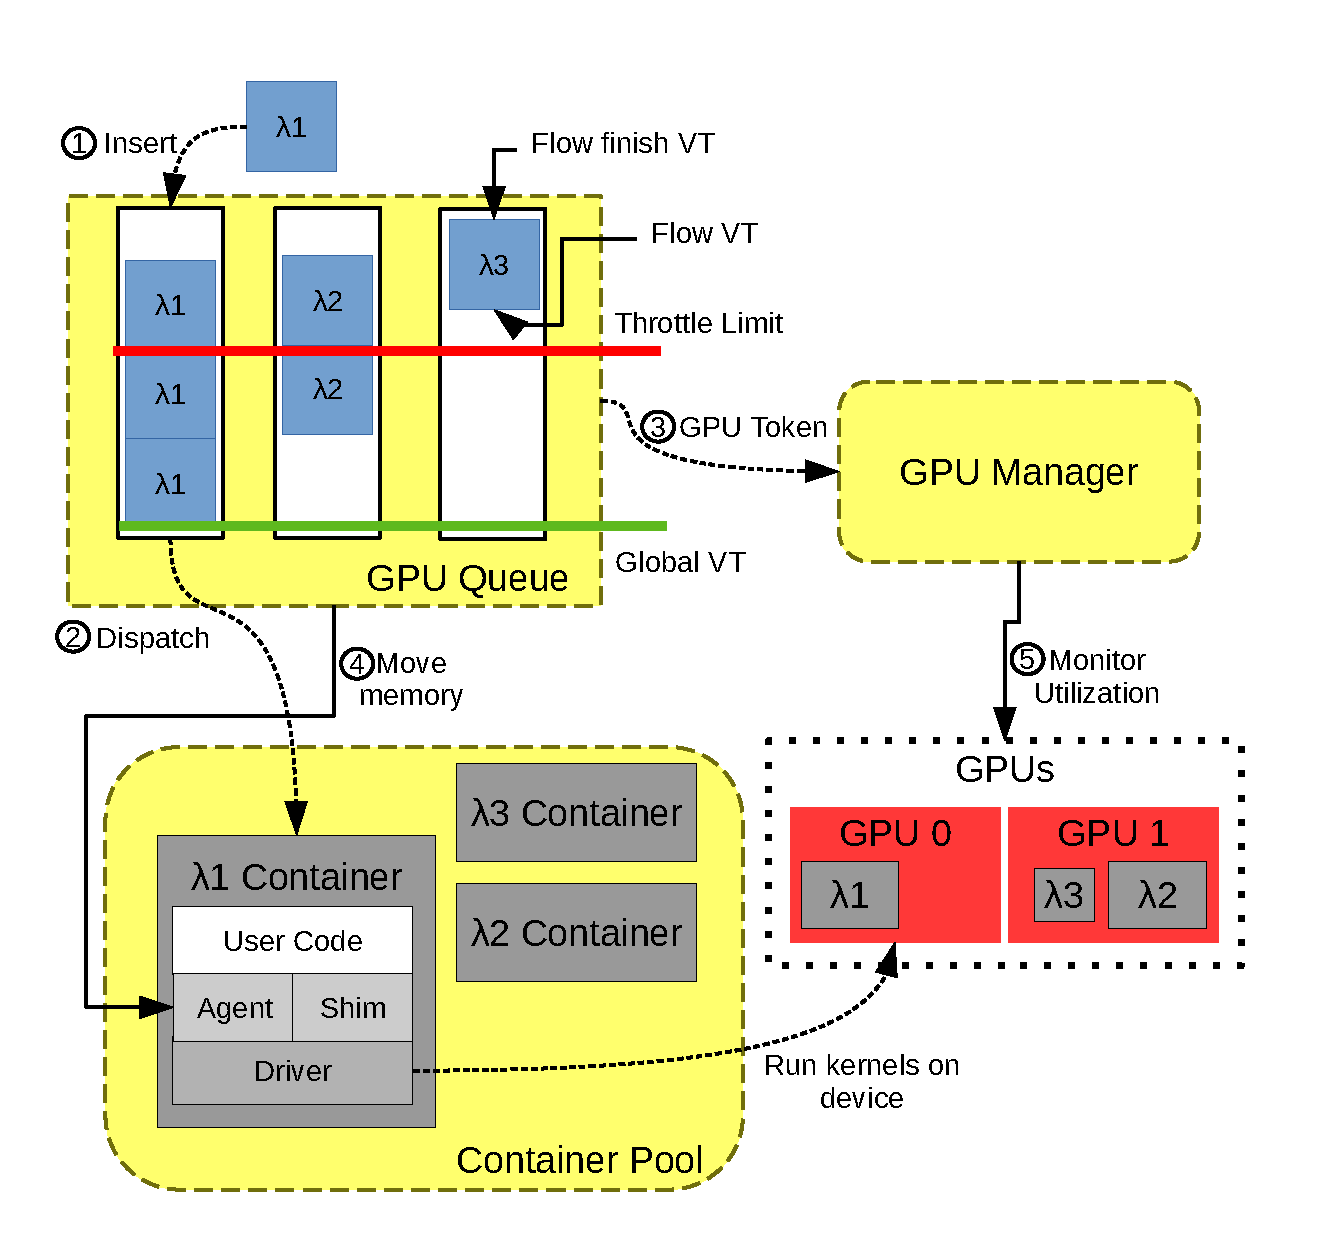
\includegraphics[width=0.9\textwidth]{mqfq/figs/queue-sys-2-simple.pdf}
  \caption{\QName~system design.}
  \label{fig:sys-diag}
\end{figure}


\subsection{Multi-Queuing}
  
% When integrating GPUs into serverless computing, we want to enable concurrent use of the device by several functions, while ensuring fairness and preventing function starvation. 
% If we want to enable several applications 
% Many applications cannot fully saturate a GPU's resources~\cite{}, and devices can often handle concurrent kernel launches from several applications
Next we delve into detail about how this new queue design can both ensure fairness and handle multiple invocations to run on one GPU.
The design of the GPU queue piece is adapted from I/O handling and queuing policies that seek to accomplish similar goals to ours, specifically Mutli-Queue Fair Queuing (MQFQ)~\cite{hedayati2019multi}.
Modern I/O devices support multiple hardware input queues that are concurrently served from, and numerous distinct processes can submit tasks to the device.
%  which was designed to maximize throughput of storage hardware that supports multiple input queues to handle requests from numerous processes.
Multi-queuing maintains state and several per-flow metadata values that avoid contention and ensure fairness between functions (called \emph{flows}), which are listed in Table~\ref{tab:mq-symbols}.

% In MQFQ, I/O requests from processes are inserted into local queues (flows) that are pinned to CPU sockets for locality.
% Each flow has a \emph{virtual time (\VT)} that is incremented on each dispatch at the core of the fairness mechanism.
% if the VT isn't too far ahead of the minimum time across all flows, is allowed to dispatch, else the flow is throttled to enforce fairness.
% A global token system limits the maximum number of in-flight requests across all flows to the device's maximum throughput, to prevent overloading.
% These two features of MQFQ, flow fairness and preventing device over-saturation, map well to the heterogeneous nature of serverless functions and avoiding GPU resource contention.
% Multi-queuing's design, shown in Figure~\ref{fig:sys-diag}, does away with the common single queue of policies like FIFO and Round Robin.
% \QNameFull's (\QName) design, shown in Figure~\ref{fig:sys-diag}, creates a unique queue, called a \emph{flow} for each function it is serving.
% Each function is given a unique \emph{flow} with new items being inserted into the top of each flow in \circled{x}.
New items are again inserted into their respective flow \circled{1}, and when a flow is non-empty, it is considered \emph{active} and only when active can be selected for dispatching.
Each flow is given a \emph{virtual time} (\VT) to be used to determine how many times flows have been served in relation to each other.
From each \VT, a global minimum \VT~(\GlobVT) across active flows is kept via a minimum indicator structure, or \emph{mindicator}.
% From each \VT, a minimum \emph{global virtual time} (\GlobVT) is computed from all active flows.

% To send an invocation to the device, MQFQ randomly
In MQFQ, each flow is managed by a separate thread, and dispatch independently of each other.
As a flow is dispatched from, its \VT~is incremented and with these the \GlobVT~also increases over time.
% To enforce fairness any flow is not allowed to have its \VT~go beyond \GlobVT~by a certain amount called \T.
Fairness is enforced by ensuring that no flow is allowed to get \T~time head of \GlobVT.
% Any flow that meets this criterion is immediately \emph{throttled}, and is not considered for dispatching until \GlobVT~has increased.
Once a flow exceeds the throttle limit, it is \emph{throttled} and cannot be dispatched from until once again its $\VT + \T < \GlobVT$.
When $\T == 1$, we get perfect fairness as any active flow cannot get more service time than any other flow.
In practice, \T~is larger to reduce coordination contention on shared data structures, while keeping flows within fairness bounds.
% As a flow is dispatched from, its \VT~is incremented and the \GlobVT~also increases over time.
Throttled flows are returned to active status as \GlobVT~grows and then may dispatch again.

After the last item from a flow is removed and completes, it transitions to \emph{inactive}, and accordingly no longer contributes to \GlobVT.
To prevent a flow from accruing credits, upon its transition from inactive to active we update $flow.\VT = max(flow.\VT, \GlobVT)$.

% To prevent overloading of the device, the queue must limit the number of in-flight dispatches, the maximum supported value of which is denoted by \D.
%  before dispatching the queue acquires a token \circled{3}
Lastly, a device can only support a limited amount of function parallelism before causing device-level throttling.
To handle this, we limit the number of per-device concurrent dispatches with \D~tokens representing permission to run on a device.
% Before formally dispatching from a flow, the queue only proceeds if a token \circled{3} is acquired.
Removing an item from a flow and sending it to the device only proceeds if a token \circled{3} is acquired.

% A dispatch thread monitors when a GPU becomes available, considers all active flows, chooses one, and removes the oldest item from it.
% The invocation is dispatched to an available container \circled{2}, and if none is present, one is created and attached to a GPU, where the item executes.
% the queue picks a flow and in \circled(2) dispatches its oldest item to start running.


\begin{table}
  \centering
  \caption{List of symbols in \QName's design.}
  \label{tab:mq-symbols}
  \begin{tabular}{c|p{6.2cm}}
    \hline
    Symbol & Description \\
    \hline
    \VT & Virtual Time, device wall clock service time of a flow \\
    \GlobVT & Minimum \VT~across all active flows \\
    \T & Amount any flow's \VT~can exceed \GlobVT~before being throttled \\
    \D & Device concurrent invocations, can be fixed or dynamic with a maximum \\
    % \FinVT & A Flows \quotes{Finish}~\VT, the flow's \VT~plus its length by average execution time \\
    TTL & Time-to-Live for an empty flow to become inactive \\
    % Service Average & Amount by which a flow's \VT~is increased after dispatch \\
  \end{tabular}
\end{table}

\subsection{\QNameFull}
\label{sec:mq}

Multi-Queuing is an excellent design for systems that must throttle unequal flows and manage external device contention.
It is insufficient to simply port the MQFQ pattern to GPUs and expect ideal performance.
The dissimilarity of their workloads must be taken into account and integrated into a new wholly new system.
GPU functions have different compute and memory footprints, execution runtimes, and importantly require state on-device for good performance: all of which diverge from disk assumptions.
GPUs cannot support the 100+ active dispatches of solid state disks~\cite{hedayati2019multi}, especially with the unknown utilization of invocations.
We modify the original MQFQ design to account for these significant deviations to get maximum performance out of our accelerator.
% Tasks sent to sold-state disk I/O use equal amounts of device time and resources.
% Their GPU function counterparts can vary widely in both of these metrics, including between invocations of the same function.
% Disks can also handle over 100 parallel requests, and GPUs see execution overhead with single-digit concurrency that also is dependent on compute and memory usage.


\mhead{Variable Execution Time}
The first difference it device dispatches no longer having the same execution time.
Without adjustment, this favors long-running functions who would get more wall time on-device because their \VT~increase is identical to smaller functions.
We therefore switch the \VT~increment to use each function's average execution time, directly correlating service time with time on device. 
Shorter functions are allowed more \emph{invocations} than their long counterparts, but each now get equally fair device time.

\mhead{Device Footprints}
% A device's concurrency limit \D~is not pre-determined as in the disk case.
% We must 
Because each function uses different amounts of compute and memory during execution, we cannot have a fixed \D~as disks do.
We track memory usage of running containers and GPU compute utilization to adjust \D~dynamically with load to minimize contention and execution overhead.
% These methods are described in detail in Sections~\ref{sec:gpu-man} and~\ref{sec:design-cont-shim}.
A shim that tracks memory usage is described in Section~\ref{sec:design-cont-shim}, and GPU manager for compute usage in Sections~\ref{sec:gpu-man}.

\begin{comment}
Not sufficient for GPU case
different 'i/o' times, variable resource usage, no locality, ignores device state, etc.

To provide these needs, locality and fairness, we need a new queue design.
Each function must track how much service time it has been given to prevent resource hogging.
Good performance can be achieved by having a function run several times in succession.
The control plane should be able to use ad-hoc and tunable heuristics to improve scheduling decisions.
All of these can be accomplished by replacing a single, flat queue with individual queues per function.


% A device can only support a limited amount of function parallelism before causing contention and device-level compute throttling.
% To handle this, we limit the number of per-device concurrent dispatches with \D~tokens representing permission to run on a device.
% Before formally dispatching from our chosen queue, we query the GPU manager \circled{3} for a token, only proceeding if one is acquired.
We cannot migrate a container between GPUs, so if existing containers do not match our GPU-specific token, we must also start a new one that does.
This manager described below in Section~\ref{sec:gpu-man} tracks utilization, dispatches, and completions, minimizing contention by dynamically changing \D~with utilization.

% Something about \D~scaling, throttling with \T\, rest of system \dots
To enforce fairness, each flow has a \emph{virtual time} (\VT), from which a global minimum VT (\GlobVT) across active flows is kept via a minimum indicator structure, or \emph{mindicator}.
After a flow is dispatched from, its \VT~is incremented by its function's average runtime. % normalized by the flow's weight.
% Choosing to use the wall time directly correlates a flow's \VT with how much service time on the GPU it has received.
Therefore, \VT~is the wall clock service time a flow has received.
This benefits smaller functions by preventing large tasks from using an outsized share of compute time. 
% Fairness is enforced by ensuring that no flow is allowed to get \T~time head of \GlobVT.
% Any flow that meets this criterion is immediately \emph{throttled}, and is not considered for dispatching until \GlobVT~has increased.

When a flow is emptied, it will be marked \emph{inactive} and ignored during dispatching.
Our mindicator removes inactive flows from consideration for \GlobVT, preventing such flows from blocking scheduling by being out-of-date. 
% Once marked inactive, that flow's containers also have their data moved off-device.
A flow moving from inactive to active after an insertion has its \VT~fast-forwarded to the current \GlobVT~to prevent them accumulating credits while idle.

We use a central dispatch thread to eliminate overhead from the control plane.
In MQFQ's disk I/O scenario, dispatches happened on the order of millions per second, and devices have internal parallelism \D~handle over one hundred outstanding I/O requests.
A GPU can be overloaded with single-digit numbers of concurrent functions, and due to their length, dispatches typically occur in the tens per second.
Having a thread for each flow monitoring when tokens are available and changes in flow \VT~has enormous overhead.
The small device parallelism also limits the potential device locality of a flow having several successive dispatches, as who gets to run becomes a quasi-random choice of the OS scheduler on which flow's thread runs first.
This design change raises its own concerns: repeatedly choosing the minimum \VT~flow for dispatching leads to MQ acting akin to FIFO, always selecting the \quotes{oldest} item across all flows.
The \quotes{sticky} portion of \QName~is our solution to this which we describe in detail next.
% Our solution to this is to have \quotes{sticky} selection of flows, which we describe in detail below in Section~\ref{sec:locality}.
\end{comment}

\mhead{Data Locality}
% Locality can have be achieved in multiple ways \dots
Function's benefit not only from having an existing container available to run in, but also from having their data on-device when they do to run.
Flows that become active have their data moved onto the device in anticipation of use \circled{4}, if space is available.
When a container is about to execute, we move all its data to the GPU to ensure it will have optimal performance.
Throttled and inactive functions immediately have their data moved off-device, because we don't expect them to run in the near future.
% Reclaiming device memory allows us to warm an active flow's data, data movement details are described in Section~\ref{sec:design-cont-shim}. 
Data monitoring and movement details are described in Section~\ref{sec:design-cont-shim}. 
% This also frees up memory for 
% When a flow is throttled, we don't expect it to run until other flows catch up, so all containers belonging to that flow have their data moved off-device to free up memory.

% Running repeatedly from a flow aids in data locality, so added several mechanisms to increase the flow dispatch locality.
% To start, a single flow is allowed to be \T ahead of the minimum flow's VT, but in the default algorithm the minimum VT flows is always chosen.
% Running repeatedly from a flow aids in data locality, which requires our dispatch algorithm to optimize for both it and fairness,
% We use several pieces of metadata from each flow to schedule, their \emph{finishing VT} \FinVT, number of enqueued items, and currently running invocations.
% The top active flows with the largest (i.e. oldest) \FinVT~are selected, targeting those flows which are most backlogged for draining.
% Using \VT~alone would likely remove flow from future consideration as only its \VT~changes, allowing other flows to take its place.
% From the top flows, the largest flow having the least number of active invocations is selected for dispatch.
% When $\D == 1$ running invocations will always be 0 during dispatch, so this devolves into a secondary sorting on flow length.
% For $\D > 1$, by sorting on active invocations we avoid concurrently running a function with itself to avoid cold starts, unless there is only one flow in which case it will be chosen.
% This selection enables repeated dispatching from a flow while still ensuring fairness by throttling a flow when its \VT~exceeds \T.
% The full dispatch algorithm is described in detail below in Section~\ref{sec:dispatch}.
% Each flow maintains a \VT and \FinVT

% instead choose the flow with the maximum \emph{finish\_vt}, draining the oldest flow until it is empty or throttled by \T.
% This choice of finishing VT is stable to cause a flow to be dispatched from successively, achieving locality.

% Being able to foresee that a function will be needed soon
The bursty and heterogeneous nature of function arrivals can cause a flow to be empty, but we can often expect a new invocation for it in the near future.
To keep data local, we add a time-to-live (TTL) timeout to each flow to prevent it becoming inactive.
An empty flow remains \emph{active} from the time of its last invocation's completion until the expiration of the TTL, then we mark it inactive.
This TTL uses each function's inter-arrival-time as a base, informed by the bursty nature of FaaS that invocations will either come frequently or after long empty periods~\cite{shahrad2020serverless}.
% Active but empty flows are of course still included when determining \GlobVT.

\subsection{Dispatch Algorithm}
\label{sec:dispatch}

The central hub of our queuing and scheduling design is the dispatching step \circled{2}, where a flow is chosen to execute next.
% Given the low number of concurrent dispatches, we have a single queue structure and associated thread for performing dispatching. 
We make our dispatcher both the primary source of locality for our queue, but also the place for fairness enforcement.
Rapidly switching between functions does not allow for reuse of data on device, but always selecting the same flow leads to starvation.

% The dispatch Algorithm~\ref{algo:dispatch} starts with acquiring a GPU token, and get the minimum VT across flows.
% If no token is received, we exit immediately as no GPU is available to run an invocation.

At the start of dispatching, we update the state of each flow in \emph{update\_state} according to the \GlobVT~in line~\ref{lst:line:update_vt}.
The first flow state update checks to see if it is and has been empty for longer than the TTL, signifying that it hasn't seen any invocations for some time.
It is marked inactive and loses any locality we had maintained, as we don't anticipate it will be used in the near future.
% If it is empty and has been for longer than the TTL, the flow is marked finally inactive.
Next, flows who match $flow.\VT + \T \ge \GlobVT$ have exceeded the throttling threshold and are immediately throttled.
Any flow that doesn't fall into these categories are kept active, may be dispatched from if non-empty, and hold onto resources.

Once states has been updated, in line~\ref{lst:line:filter} we consider for dispatch all flows both active and non-empty.
% To enable stickiness, we develop a multi-stage selection inspired by Power of Two Choices~\cite{mitzenmacher2001power}.
% In addition to a \VT, flows have a corresponding \FinVT~computed as the \VT~plus the average execution time multiplied by the number of enqueued items.
% We order active and non-empty flows by their \FinVT~and select the top $max(0.3*num\_active\_flows, \D)$ flows.
% The maximum here allows us to have the top set of flows to consider between, increasing the consideration set with \D~to allow more flows to concurrently dispatch.  
From this subset we must choose a single flow, using a piecewise function on \D~for best performance.
When $\D == 1$, the flow with the most number of enqueued items is picked.
% Otherwise we choose the flow with the least number of currently executing invocations breaking ties using the longest length again.
When $\D > 1$ we still select on queue length, but on~\ref{lst:line:in_flight} break ties in the favor of the flow with the least number of currently executing invocations.
This encourages multiple flows to progress and reduces the chance of a cold start caused by concurrent execution of the same function.
In both cases we are draining the most backed up queues and enabling flow stickiness.
If no token is received, we return \texttt{None} as no GPU is available to run an invocation.
The flow that is ultimately chosen is returned at~\ref{lst:line:done}, a token to run on GPU is acquired, and the flow's oldest item is removed and sent out to be executed.
% Our selection of the flow with the largest \FinVT~allows dispatches to continue from non-empty flows, and we accept the unlikely scenario of all flows being throttled while an old and empty flow waits to expire.

\algnewcommand{\LineComment}[1]{\State \(\triangleright\) #1}
\begin{algorithm}[H]
\begin{algorithmic}[1]
\caption{Flow Dispatching Algorithm}
\label{algo:dispatch}
\Procedure{Dispatch}{}
\State $\GlobVT \gets mindicator.min()$
\State $chosen \gets None$
\For{$flow \in flows $}
\State $update\_state(flow, \GlobVT)$ \label{lst:line:update_vt} %\Comment {Set Inactive/Throttled}
% \If{$flow.is\_active() \textbf{ and } !flow.is\_empty()$}
%   \If{$chosen == None$}
%     \State $chosen \gets flow$
%   \ElsIf{$chosen.finish\_vt < flow.finish\_vt$}
%     \State $chosen \gets flow$
%   \EndIf
% \EndIf
\EndFor
% \State $to\_select \gets max(3, \D)$
% \State $sort(flows, on: \FinVT)$
% \State $flow\_cnt \gets max(0.3*num\_active\_flows, \D)$
% \State $candidates \gets top(flow\_cnt, flows)$
\State $cand \gets filter(flow.active~\textbf{and}~flow.len > 0, flows)$ \label{lst:line:filter}
\State $sort(cand, on: length)$
% \State $chosen \gets max(candidates, on: length)$
\If{$\D \ne 1$}
\State $sort(cand, on: in\_flight)$ \label{lst:line:in_flight}
\EndIf
\State $chosen \gets top(cand)$
\State $token \gets get\_token(chosen)$
\If{$token == None$}
\State \Return $None$
\EndIf
\State $mindicator.update\_vt(chosen)$
\State \Return $chosen.pop()$ \label{lst:line:done}
\EndProcedure
\\
\LineComment{Update state of flow, given the global \VT}
\Procedure{update\_state}{flow, \GlobVT} \label{lst:line:update_state}
\If{$flow.is\_empty~\textbf{and}~flow.in\_flight==0$}
\If{$Date.Now() - flow.last\_exec \ge TTL$}
\LineComment{Flow has expired}
\State $flow.state \gets Inactive$
\EndIf
\ElsIf{$flow.\VT - \GlobVT < \T$}
  \LineComment{Flow has exceeded threshold}
  \State $flow.state \gets Throttled$
\Else
\State $flow.state \gets Active$
\EndIf
\EndProcedure
\end{algorithmic}
\end{algorithm}

\subsection{Memory Overcommitment}
\label{sec:design-cont-shim}

Each container has a custom shim that intercepts calls to the GPU driver, specifically those for initialization and memory allocations.
Requests by functions to allocate physical memory are captured in and converted into UVM (virtual device memory) allocations, allocation metadata is stored, and the result is returned to function.
When some flow becomes active, the queue, via our agent inside each container, directs the shim to move the memory for the flow's containers onto the device in anticipation of use \circled{4}.
In the event memory pressure is too high, this is delayed until an invocation is about to be dispatched, and only the container about to execute migrates memory.
When a function's flow is inactive or throttled, we again use the shim to move container memory off the device to free up space.
Because our shim tracks memory metadata, we can know how much memory a container needs on-device, and our GPU monitor ensures we don't over-subscribe memory with running invocations.
% Our driver can move the memory on and off the device to ensure

\subsection{GPU Load Management}
\label{sec:gpu-man}

The GPU monitor is responsible for two key mechanisms: tracking GPU assignment and monitoring GPU utilization \circled{5}.
Creating a GPU context uses physical memory we can't control, so the monitor only allows a fixed number of containers to exist at one time.
New containers are launched on the GPU with the most available slots and mapped to the device they are assigned.
When is required but not available, we use this mapping to evict a container to make room.
% When a slot isn't available, we use this mapping to evict a container using an LRU caching strategy to get a slot on the device that we want to run on from Section~\ref{sec:design}.

GPUs have limited memory and compute, and if we don't monitor how much function's use, they can interfere with each other and increase execution latency.
This limited number of concurrently executing functions is captured in \D, and is the primary mechanism of the control plane to prevent interference.
\D~can be either a fixed maximum value, or dynamically adjusted by the control plane at runtime.

Dynamically setting \D~is dependent on the two main resource limitations of GPUs, on-device physical memory and compute.
Because we intercept memory allocations, we can closely track device memory usage of containers thanks to our driver shim, and only allow a new dispatch when the needed container won't overload the device's physical memory.
Ensuring there is available compute is not as straightforward to manage as memory due to unpredictable function characteristics.
An ML inference task for example could have known compute usage, who's input and weight tensors will have fixed compute uses based on some execution graph.
Other types of GPU functions can launch compute kernels unpredictably, based on the application's internal control flow.
The actual size and number of kernel launches often vary with function arguments, making an a priori utilization intractable.
Accepting this, we choose to externally monitor device utilization and launch new invocations when headroom is deemed sufficient to support another dispatch.
To avoid a thundering herd of launches, we increment the tracked usage by a factor of $1/\D$, and let the next monitoring update capture actual usage.
When both resources are deemed available for a dispatch, we \quotes{increase} \D~by allowing the item to start executing.
Our active management of both resources changes the nature of \D~from a fixed parallelism limit to a dynamic runtime control knob.
% Tracking both container/GPU mapping, and GPU utilization to allow function to start running

